% \VignetteIndexEntry{spcopula: Modelling Spatial and Spatio-Temporal Dependence with Copulas in R}

\documentclass[article,nojss]{jss}
%\Month{month}
%\Year{year}
%\Volume{vol}
%\Issue{issue}
%\Submitdate{2013-06-01}
%\Acceptdate{2012-09-26}

\usepackage[utf8]{inputenc}
\usepackage{alltt}
\usepackage{graphicx}
\usepackage{amssymb}
%% \usepackage{amsthm}
\usepackage{amsmath}

%% extra packages
\usepackage{array}
\newcolumntype{L}[1]{>{\raggedright\let\newline\\\arraybackslash\hspace{0pt}}p{#1}}
\usepackage{enumitem}
%%



\author{Benedikt Gr\"{a}ler}

\title{\pkg{spcopula}: Modelling Spatial and Spatio-Temporal Dependence with Copulas in \proglang{R}}

\Plainauthor{Benedikt Gr{\"a}ler} %% comma-separated
\Plaintitle{The spcopula R package: Modelling Spatial and Spatio-Temporal Dependence with Copulas} %% without formatting
\Shorttitle{Spatio-Temporal Vine Copulas}

\Address{
Benedikt Gr\"{a}ler\\
Institute for Geoinformatics\\
University of M\"{u}nster\\
Heisenbergstr. 2\\
48149 M\"{u}nster, Germany\\
E-mail: \email{ben@graeler.org}\\
URL: \url{http://ben.graeler.org}}

\Abstract{
The \pkg{spcopula} \proglang{R}~package provides tools to model spatial and spatio-temporal phenomena with \emph{spatial} and \emph{spatio-temporal vine copulas}. Copulas allow us to flexibly build multivariate distributions with mixed margins where the copula describes the multivariate dependence structure coupling the margins. In classical geostatistics, a multivariate Gaussian distribution is typically assumed and dependence is summarized in a covariance matrix implying limitations like elliptical symmetry in the strength of dependence. Copulas allow for dependence structures beyond the Gaussian one, being for instance asymmetric. We developed the spatio-temporal vine copulas such that the bivariate copula families in the lower trees may change with distance across space and time allowing not only for a varying strength of dependence but also for a changing dependence structure. These spatio-temporal distributions are used to predict values at unobserved locations, assess risk, or run simulations. Based on the concept of vine copulas, the \pkg{spcopula} package provides a large set of multivariate distributions. As bivariate spatial copulas do not have any probabilistic restrictions, the spatial vine copula is a powerful approach for modelling skewed or heavy tailed data with complex and potentially asymmetric dependence structures in the spatial and spatio-temporal domain.}

\Keywords{spatial data, multivariate distributions, spatial modelling, interpolation}

\graphicspath{{figures/}}

\usepackage{Sweave}
\begin{document}
\Sconcordance{concordance:spcopula.tex:spcopula.Rnw:%
1 49 1 1 0 1 1 1 5 72 1 1 18 109 1 1 2 1 0 1 5 7 0 1 2 9 1 1 2 %
4 0 2 2 4 0 1 2 8 1 1 4 6 0 1 2 1 3 5 0 1 2 4 1 1 4 6 0 1 2 17 %
1 1 5 4 0 1 1 3 0 1 2 1 5 4 0 1 1 3 0 1 2 2 1 1 3 5 0 1 2 3 1 %
1 3 2 0 1 1 3 0 1 2 3 1 1 2 4 0 1 2 2 1 1 2 4 0 1 2 2 1 1 2 1 %
0 1 1 3 0 1 2 2 1 1 2 4 0 1 2 2 1 1 5 4 0 1 1 1 2 4 0 1 2 60 1}

\maketitle

%\tableofcontents

\section{Introduction}
\label{sec:introduction}

Interpolation of spatial random fields is a common task in geostatistics. Simple approaches like inverse distance weighted predictions or the well known kriging procedures have routinely been applied for many years. However, when the underlying assumptions (i.e., a multivariate Gaussian distribution, possibly after transformation) of these approaches are hard to be fulfilled, alternatives are needed. Copulas have been used in some applications in the domain of spatial statistics. \citet{Bardossy2006} was one of the first to apply copulas in a geostatistical context. Some recent advances incorporating copulas in this field have for instance been published by \citet{Kazianka2011,Kazianka2010}, \citet{Bardossy2011}, \citet{Bardossy2009} or \citet{Bardossy2008}. They use a comparatively small set of copula families to model spatial processes. 

The spatio-temporal domain rises in interest since several years, and several extensions of the spatial approaches to spatio-temporal ones have been developed \citep[see e.g., ][]{Cressie2011}. A major challenge with extending spatial kriging to spatio-temporal kriging is to build and fit well defined spatio-temporal covariance functions. The approach presented here differs from the classical geostatistical ones by using \emph{spatio-temporal vine copulas} to build a spatio-temporal distribution that does not rely on the Gaussian assumption, nor involves a covariance matrix. It extends the spatial vine copula \citep{Graler2014} to the spatio-temporal context. Similar to co-kriging, we will introduce a spatio-temporal vine copula approach incorporating covariates.

The advantage of the \emph{spatio-temporal vine copula} is its flexibility in the selection of copula families through \emph{bivariate spatio-temporal copulas}. Bivariate spatio-temporal copulas are a convex combination of different copula families that are parameterised by spatial and temporal distance (Equation~\ref{eq:spCop} in Section~\ref{sec:stVineCop}). This changing dependence structure allows for instance to preserve spatial symmetry within each time step while allowing for a directional effect across time. The introduction of a \emph{bivariate spatial copula} into a vine copula for interpolation has been described by \citet{Graler2014}. The bivariate spatial or spatio-temporal copulas are combined into a \emph{vine copula} \citep[initially called \emph{pair-copula construction} by][]{Aas2009,Bedford2002} for a local spatial or spatio-temporal neighbourhood. A first approach to extend the spatial to the spatio-temporal approach has been presented in \citet{Graler2012a}. This paper describes a more flexible spatio-temporal neighbourhood structure and the introduction of a covariate to improve the prediction. Adding marginal distributions to the spatial or spatio-temporal vine copula yields a full multivariate distribution describing a local distribution of the observed phenomenon. 

The \pkg{spcopula} \proglang{R}~package provides functions and classes to model spatial and spatio-temporal phenomena by vine copulas. Different tools have been implemented to fit spatial and spatio-temporal vine copulas to a data set, to interpolate the random field, and to predict quantiles from it. The package extends the \pkg{copula} \proglang{R}~package \citep{Kojadinovic2010a,Yan2007} and provides additional copula families. Wrapper classes following the \pkg{copula} design to the copula families available in \pkg{VineCopula} \citep{Schepsmeier2013} that have been implemented in \pkg{spcopula} are now directly available in \pkg{VineCopula}. The functionality for non-spatial vine copulas relies on \pkg{VineCopula}. For handling spatial and spatio-temporal data, \pkg{spcopula} builds on the \proglang{R}~packages \pkg{sp} \citep{Pebesma2005} and \pkg{spacetime} \citep{Pebesma2012}. A more detailed overview of core dependencies and contributions of \pkg{spcopula} is provided in Table~\ref{tab:contribution}.


\begin{table}
\small
\setlength{\itemsep}{-2pt}
\centering
\begin{tabular}{l|L{0.35\textwidth} L{0.45\textwidth}}
Package & \pkg{spcopula} reuses and extends & \pkg{spcopula} adds to the functionality \\ \hline
\pkg{copula} &
\begin{itemize}[leftmargin=*, noitemsep, nosep]\vspace{-\baselineskip}
\item S4-class definition \code{copula}
\item methods \code{fitCopula}, \code{dCopula}, \code{pCopula}, \code{rCopula}\vspace{-0.9\baselineskip}
\end{itemize} & 
\begin{itemize}[leftmargin=*, noitemsep, nosep]\vspace{-\baselineskip}
\item bivariate copula families \code{asCopula}, \code{cqsCopula} and \code{tawn3pCopula}
\item empirical and analytical tail dependence functions \code{empTailDepFun} and \code{tailDepFun}
\item partial derivatives via methods \code{dduCopula} and \code{ddvCopula}
\item inverse of partial derivatives via methods \code{invdduCopula} and \code{invddvCopula}
\item inverse of bivariate copulas for a given $u$ or $v$ via methods \code{qCopula_u} and \code{qCopula_v}\vspace{-0.9\baselineskip}
\end{itemize} \\
\pkg{VineCopula} &
\begin{itemize}[leftmargin=*, noitemsep, nosep]\vspace{-\baselineskip}
\item function \code{BiCopSelect}
\item S4-class wrapper \code{vineCopula}\vspace{-0.9\baselineskip}
\end{itemize} & 
-/- \\
\pkg{sp} &
\begin{itemize}[leftmargin=*, noitemsep, nosep]\vspace{-\baselineskip}
\item abstract S4-class definition \code{Spatial}
\item function \code{spDists}\vspace{-0.9\baselineskip}
\end{itemize} & 
\begin{itemize}[leftmargin=*, noitemsep, nosep]\vspace{-\baselineskip}
\item nearest spatial neighbour calculation via function \code{getNeighbours}\vspace{-0.9\baselineskip}
\end{itemize} \\
\pkg{spacetime} &
\begin{itemize}[leftmargin=*, noitemsep, nosep]\vspace{-\baselineskip}
\item abstract S4-class definition \code{ST}\vspace{-0.9\baselineskip}
\end{itemize} & 
\begin{itemize}[leftmargin=*, noitemsep, nosep]\vspace{-\baselineskip}
\item nearest spatio-temporal neighbour calculation via function \code{getStNeighbours}\vspace{-0.9\baselineskip}
\end{itemize}
\end{tabular}
\caption{Overview of core dependencies and contributions of \pkg{spcopula}.\label{tab:contribution}}
\end{table}

The remainder of this paper is organized as follows. The theoretical background of copulas, bivariate spatial copulas, bivariate spatio-temporal copulas and vine copulas are addressed in the next section. A strategy to estimate spatio-temporal vine copulas is given in Section~\ref{sec:estimation}. Section~\ref{sec:predSim} discusses different applications of the multivariate distribution such as the possibility to predict values at unobserved locations or simulate from the spatial or spatio-temporal random field. One application is illustrated in Section~\ref{sec:application}, where daily mean $\rm{PM}_{10}$ concentrations (particulate matter less than 10 $\mu m$ in diameter) across Europe observed throughout the year 2005 are interpolated including an additional covariate. Results are discussed in Section~\ref{sec:discussion}. Conclusions are drawn in Section~\ref{sec:conclusion}.

\newpage

\section{Spatio-temporal vine copulas}
\label{sec:stVineCop}
In the following, we assume a spatio-temporal random field $Z:\Omega \times \mathcal{S} \times \mathcal{T} \rightarrow \mathbb{R}$ defined over some spatial domain $\mathcal{S}$ and temporal domain $\mathcal{T}$ of interest and an underlying probability space $\Omega$. Typically, a sample $\mathbf{Z} = \big(z(s_1,t_1),\dots,z(s_n,t_n)\big)$ has been observed at a set of distinct spatio-temporal locations $(s_1, t_1), \dots, (s_n,t_n) \in \mathcal{S}\times \mathcal{T}$ where in general some spatial locations have been sampled at multiple time instances. Often, one is interested in modelling $Z$ from the sample $\mathbf{Z}$ in order to predict at unobserved locations in space and time or simulate from the distribution. The spatio-temporal random field might as well be accompanied by a co-variate $Y$ leading to a bivariate spatio-temporal random field: $(Z,Y):\Omega \times \mathcal{S} \times \mathcal{T} \rightarrow \mathbb{R}^2$.

Copulas describe the dependence between the margins of multivariate distributions. \citet{Sklar1959} proved that any $n$-variate distribution $H$ can be split into its margins $F_1,\dots,F_n$ and the copula $C$ which couples the margins with a given dependence structure: 
$H(x_1,\dots,x_n)=C_n\big(F_1(x_1),\dots, F_n(x_n)\big)$.
A copula can be imagined as a multivariate cumulative density distribution with uniform margins where its density reflects the strength of dependence between the margins. Many different parametric copula families exist allowing for very different dependence structures including certain symmetry properties but as well asymmetric, directional influences. In a bivariate symmetric case, the strength of dependence, i.e., the copula density (denoted by $c$), of a pair $(u,v) \in [0,1]^2$ does not depend on the order, i.e., $c(u,v)=c(v,u)$, $\forall \ (u,v) \in [0,1]^2$ while this does not hold for an asymmetric copula. Thinking of $u$ and $v$ as cumulative distribution values of two consecutive time steps, this allows to model a sudden rise in value with a different strength of dependence than a sudden drop. For further details we refer to the introductory book by \citet{Nelsen2006}.

Sklar's Theorem is true for any dimension $d \geq 2$, but we will at first only consider bivariate copulas $C:[0,1]^2\rightarrow[0,1]$. The density of a copula expresses the strength of dependence which changes over the range of the marginal distributions. The only copula exhibiting a constant strength of dependence across its margins is the product copula $\Pi$ describing independence. Commonly, strength of dependence in a bivariate setting is measured by the correlation (or covariance) between two random variables and a Gaussian distribution is typically assumed implicitly. As a Gaussian distribution can be decomposed into a Gaussian copula with Gaussian margins, one imposes the Gaussian dependence structure which is elliptically symmetric (following the notion of elliptical contours of the bivariate Gaussian distribution). Hence, by only investigating the correlation of two variables, potential deviations of dependence from the Gaussian elliptical model are neglected. Different copulas might reflect samples having identical correlation, but different dependence structure (Figure~\ref{fig:copula_densities}). The same applies to the spatial and spatio-temporal domain where kriging implicitly assumes a Gaussian dependence structure. However, looking into different data sets and investigating pairwise scatter plots reveals non-Gaussian dependence structures. Especially the correlation structure of pairs spanning across time may exhibit an asymmetric (directional) dependence. Such structures can be captured by copulas.


\begin{figure}
\center
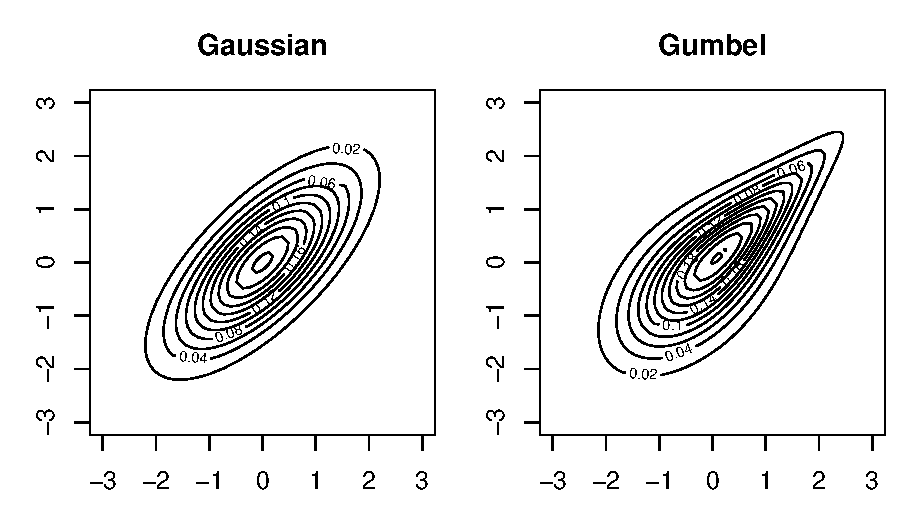
\includegraphics[width=0.8\textwidth]{copula_densities.pdf}
\caption{Copula densities of the Gaussian and Gumbel copulas. Both copulas are shown with standard normal distributed margins and a Kendall's tau correlation of 0.5.}\label{fig:copula_densities}
\end{figure}

Copulas allow to model the dependence structure of a multivariate distribution disjoint from the marginals. This introduces a huge flexibility and eases the estimation at the same time. As the analytically known multivariate copula families are rather limited in their flexibility, we use vine copulas that allow to flexibly build multivariate copulas by any combination of bivariate ones. For a successful model it is important to obtain good fits of both, margins and copula. The fitting of the margins can be carried out with any approach available in the literature. For the subsequent development of spatio-temporal vine copulas, we assume to have marginal distributions $F_{q,r}$ of $Z$ and $G_{q,r}$ of $Y$ for any location $(s_q,t_r) \in \mathcal{S}\times\mathcal{T}$.

We briefly introduce \emph{bivariate spatial copulas} as in \citet{Graler2014} by incorporating distance as the only parameter but utilizing the flexibility of many bivariate copula families. For pairs of locations we assume that the separation distance of these is the driving parameter determining the dependence. Hence, pairs of locations very close to each other are likely to exhibit a dependence structure close to perfect dependence where noise might reduce the strength of dependence to some degree (analogous to the nugget effect in kriging). For large distances, the pairs will tend to be independent and are modelled by the product copula $\Pi$. The approaches by \citet{Bardossy2011} and \citet{Kazianka2010} allow only for a single multivariate copula family. The bivariate spatial copula $c_h(u,v)$ recalled here is designed as a convex combination of bivariate copulas (in terms of their densities) that is not limited to a single family (Equation~\ref{eq:spCop}). Hence, we allow not only for a varying strength of dependence but also for a dependence structure changing with distance: 
\begin{equation}\label{eq:spCop}
c_{h} (u,v) := \left\{
\begin{array}{ll}
c_{1,h}(u,v) &, 0 \leq h < l_1 \\
(1-\lambda_2) c_{1,h}(u,v) + \lambda_2 c_{2,h}(u,v) &, l_1 \leq h < l_2 \\
\vdots & \vdots \\
(1-\lambda_k) c_{k-1,h}(u,v) + \lambda_k\cdot 1 &, l_{k-1} \leq h < l_k \\
1 &, l_k \leq h 
\end{array}
\right.
\end{equation}
where $\lambda_j := \frac{h-l_{j-1}}{l_j-l_{j-1}}$ is a linearly interpolated weight, $h$ denotes the separating distance and $l_1,\dots,l_k$ denote chosen distances of spatial bins (e.g., midpoint or mean distance of all point pairs involved in the estimation). The parameters of the copulas $c_ {i,h}$ in the convex combination may as well depend on the distance $h$. With the help of the marginal CDF or a rank order transformation, the arguments $u$ and $v$ are the values of the pairs of locations transformed to $[0,1]$. Inspecting Equation~\ref{eq:spCop} reveals that different choices of bins will in general yield different approximations to the underlying spatial dependence structure. This binning faces the same balancing issue as a classical variogram estimation where many bins allow for a flexible model but too few observations per bin and conversely few but well filled bins reduce the flexibility. It is important to maintain enough pairs per bin to allow for a sensible copula family selection throughout the estimation process.

The temporal extension of the bivariate spatial copula is yet another convex combination of bivariate spatial copulas $c_h^\Delta$ at different time lags $\Delta$. In the case where one does not want to predict the spatio-temporal random field between time steps, the bivariate spatio-temporal copula can be reduced to a piecewise defined copula where the temporal lag between both spatio-temporal locations selects the bivariate spatial copula to be used.

Concentrating on a local neighbourhood of $d$ spatio-temporal neighbours (Figure~\ref{fig:stNeigh}), we now model the pair-wise dependence between locations through a bivariate spatio-temporal copula. However, these copulas need to be joined to benefit from the full $d$-dimensional distribution of the neighbourhood. A technique to combine bivariate copulas into multivariate copulas has been introduced by \citet{Aas2009} building on work from \citet{Bedford2002}. This approach has first been introduced as the \emph{pair-copula construction} and the resulting copulas are now known as \emph{vine copulas} in the literature.

\begin{figure}
\center
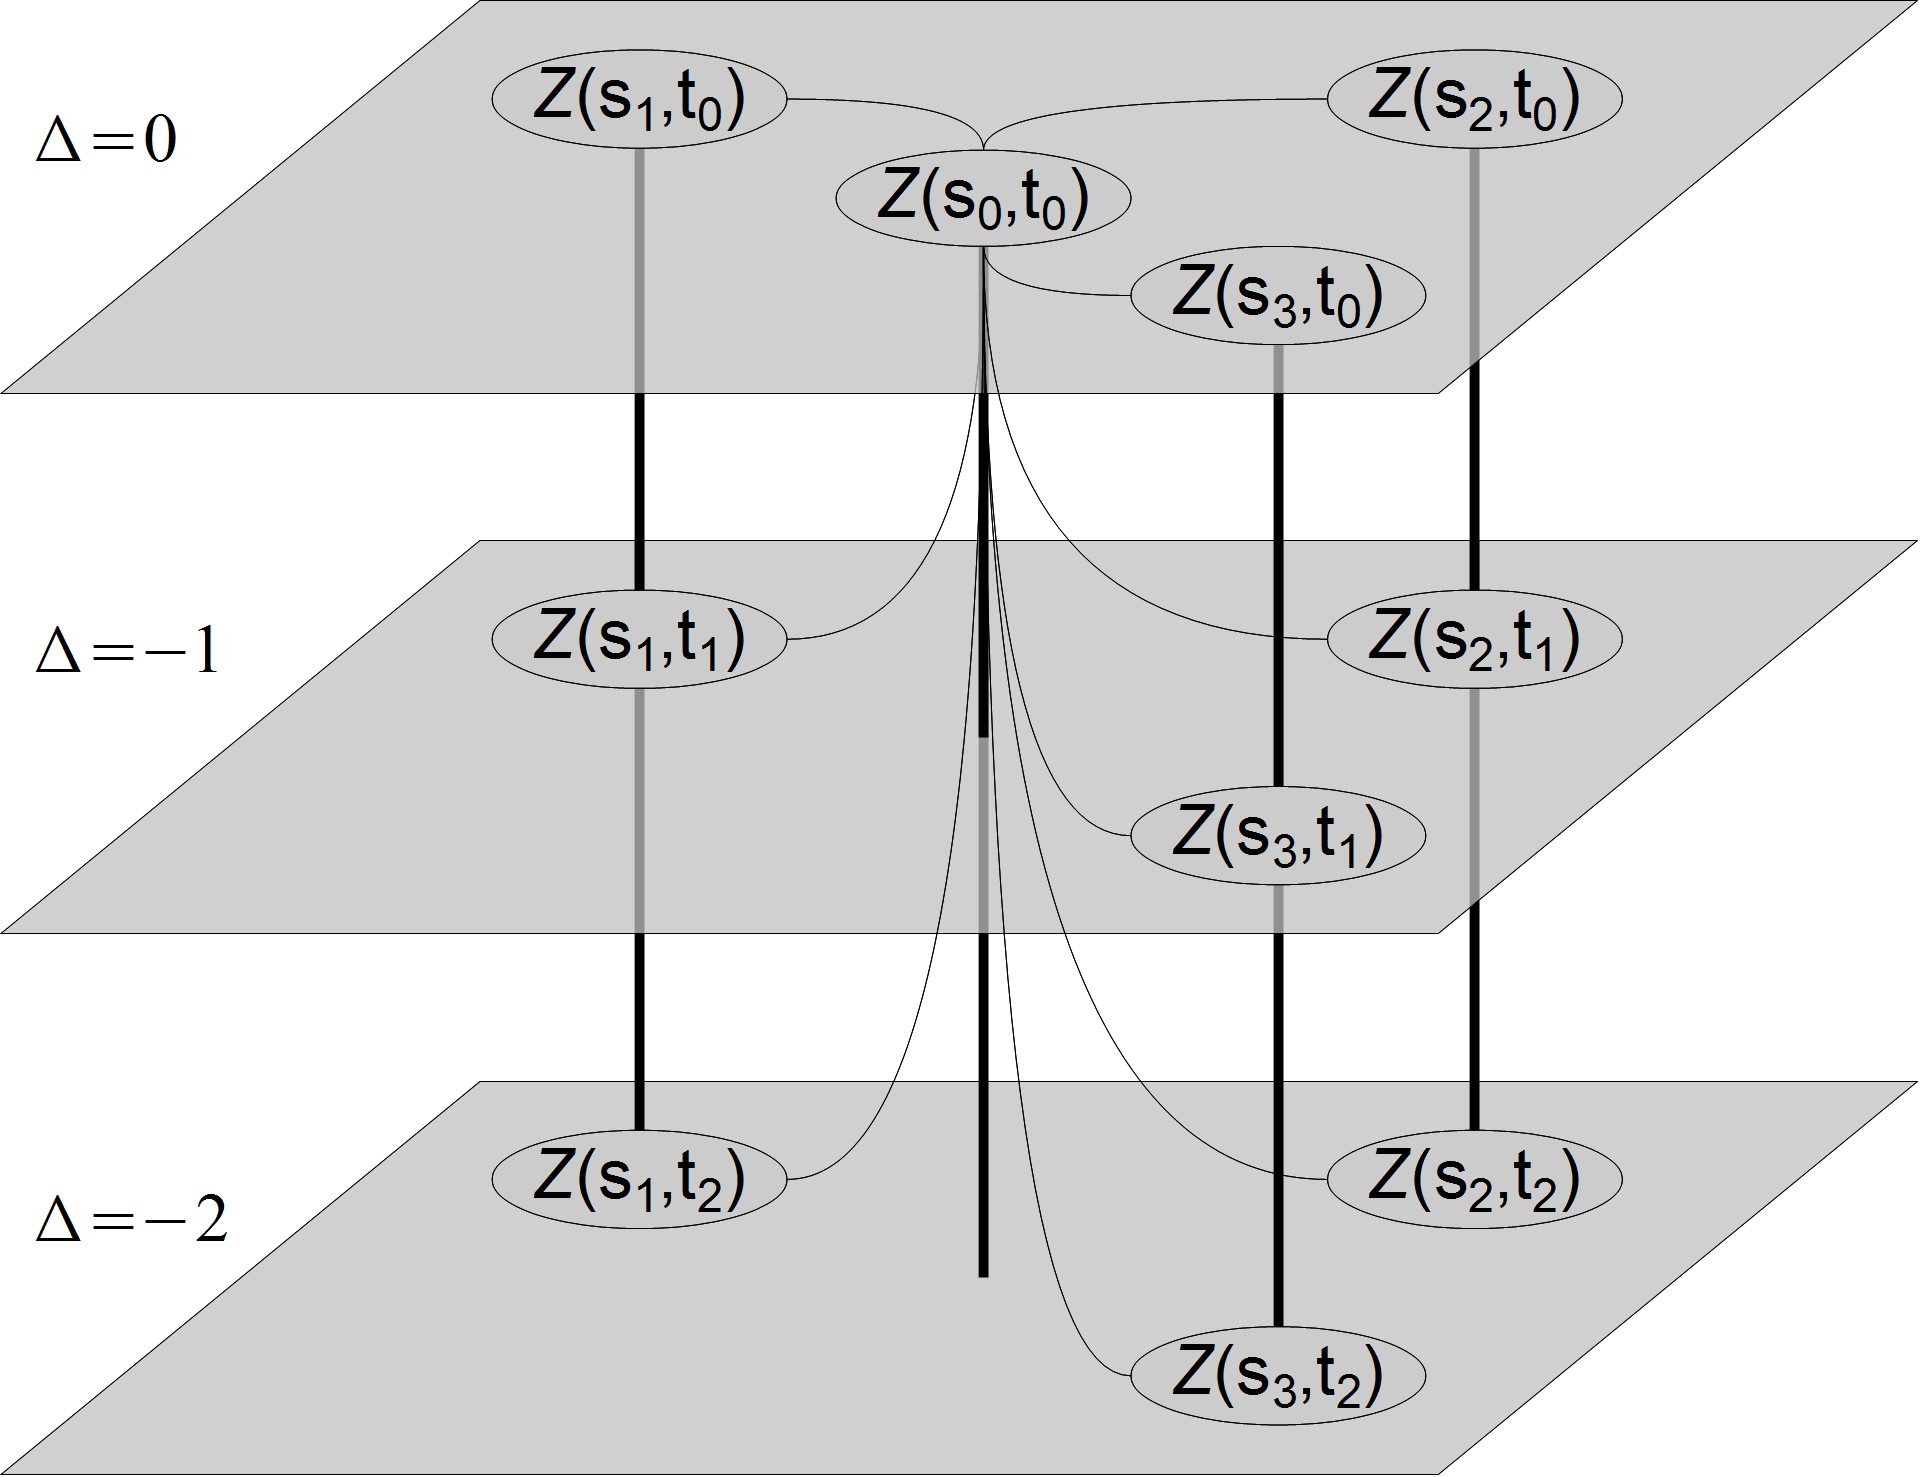
\includegraphics[width=0.49\textwidth]{st-vine.png} % 0.9*1920/3544=0.49 times the size of the can_Vine.png
\caption{A spatio-temporal neighbourhood including the three spatially closest neighbours at three different time lags.\label{fig:stNeigh}}
\end{figure}

Vine copulas approximate multivariate copulas through bivariate building blocks (Figure~\ref{fig:canVine}). The joint density is obtained as the product of all bivariate copula densities involved. In the special case of spatio-temporal vine copulas with an additional covariate $Y:\mathcal{S} \times \mathcal{T} \rightarrow \mathbb{R}$, we model the first tree by bivariate spatio-temporal copulas $c_{h}^\Delta$ and $c_{ZY}$, the copula describing the dependence between $Z$ and $Y$. The remaining upper trees are modeled by $c_{j,j+i|0,\dots,j-1}$ fixed over space and time:

\begin{align}\label{eq:spCopCoVDensity}
& c^{\mathbf{\Delta}}_{\mathbf{h}} (u_0, v_0, u_1,\dots,u_{d}) \nonumber \\ 
=& c_{ZY}(u_0,v_0) \cdot \prod\limits_{i=1}^{d} c^\Delta_{h(0,i)}(u_0,u_i) 
\cdot \prod\limits_{i=1}^{d}c_{Y,i|0} (u_{Y|0}, u_{i|0}) \nonumber \\
&\cdot \prod\limits_{j=1}^{d-1}\prod\limits_{i=1}^{d-j}c_{j,j+i|Y,0,\dots,j-1} (u_{j|Y,0,\dots,j-1}, u_{j+i|Y,0,\dots,j-1})
\end{align}

where $v_0 = G_{0}\big(Y(s_0,t_0)\big)$ with $G_{0}$ being the co-variate's $Y$ marginal cumulative distribution function at $(s_0,t_0)$, $u_i = F_i\big(Z(s_q,t_r)\big)$ for $0 \leq i \leq d$ with $(s_q,t_r)$ denoting the $i$-th closest neighbor of $(s_0,t_0)$ with marginal cumulative distribution function $F_i=F_{q,r}$. For the spatio-temporally fixed upper part of the vine it is
\begin{align}
u_{Y|0} &= F_{Y|0}(v_0|u_0) = \frac{\partial C_{Z,Y}(u_0,v_0)}{\partial u_0}\nonumber \\
u_{i|0} &= F_{i|0}(u_i|u_0) = \frac{\partial C_{h(0,i)}^\Delta(u_0,u_i)}{\partial u_0}\label{eq:pseudoObs}\\
\end{align}
\begin{align*}
u_{j+i|Y,0,\dots, j-1} &= F_{j+i|Y,0,\dots j-1}(u_{j+i}|v_0,u_0,\dots, u_{j-1})\\
	&=\frac{\partial C_{j-1,j+i|Y,0,\dots j-2}(u_{j-1|Y,0,\dots j-2},u_{j+i|Y,0,\dots j-2})}{\partial u_{j-1|Y,0,\dots j-2}}
\end{align*}
for $1 \leq j < d$ and $0 \leq i \leq d-j$.

\begin{figure}
\center
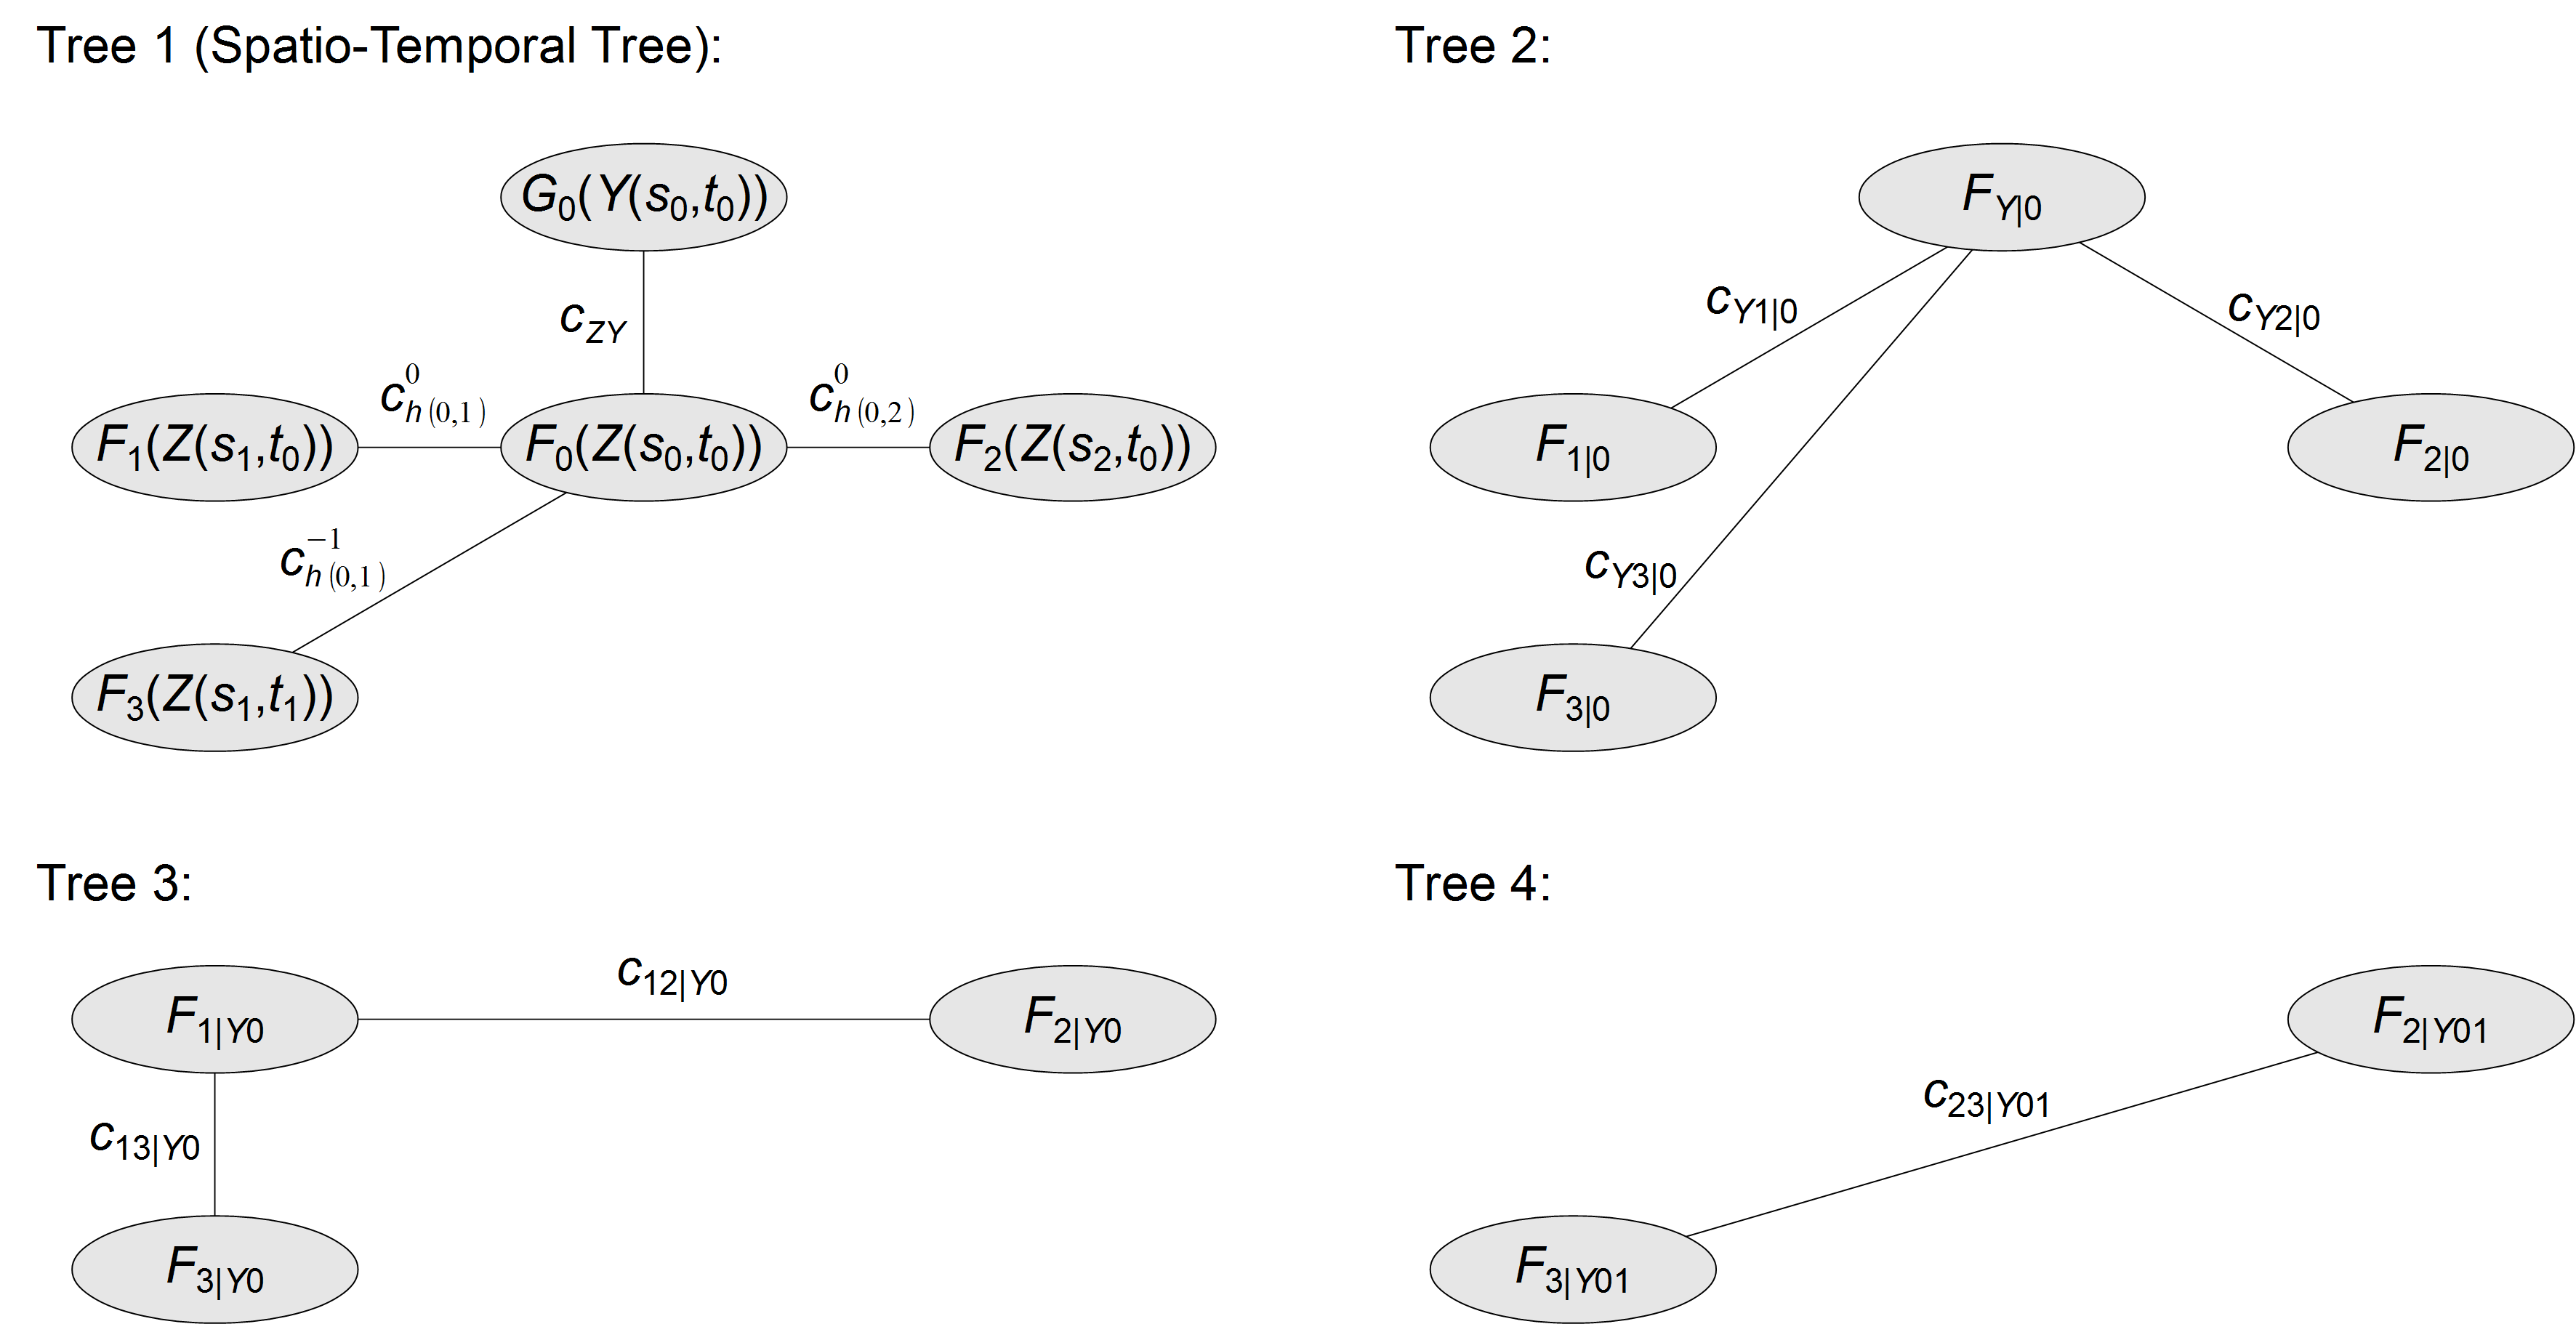
\includegraphics[width=0.9\textwidth]{can_Vine.png}
\caption{Graphical representation of a 5-dimensional local spatio-temporal vine copula with covariate $Y$, reoccurring location $s_1$ at the current and one preceding time slice and location $s_2$ at the current time slice. The notation follows the one introduced in Equation~\ref{eq:spCopCoVDensity}.\label{fig:canVine}}
\end{figure}

In general, different decompositions of a multivariate copula exist, refereed to as regular vines, but in the spatial or spatio-temporal interpolation where a central element is naturally identified, we use a canonical vine where all initial dependencies are with respect to the central location. In the spatio-temporal tree (first tree in Figure~\ref{fig:canVine}) of the spatio-temporal vine, all edges connecting different spatio-temporal neighbours are modelled through a spatio-temporal copula $c^\Delta_{h(0,q)}$ parametrized by the spatial distance $h(0, q)$ and temporal lag $\Delta=t_0-t_r$ between the data locations $(s_0,t_0)$ and $(s_q,t_r)$. The edge connecting the central location with its co-located covariate $Y(s_0,t_0)$ is represented by the best fitting bivariate copula $c_{ZY}$. In general, the dependency between the variable of interest and its covariate might as well change over space and time. All consecutive upper trees are modelled through spatio-temporally constant copulas. The upper vine structure does not impose any restriction on the bivariate copulas involved and are kept fixed no matter how the neighbourhood might be organized. The conditional distribution functions given in the above equations can immediately be obtained as partial derivatives of the already modelled copulas. 

To achieve a full distribution describing the local behaviour of the spatio-temporal random field $Z$, margins need to be joined with the spatio-temporal vine copula. Depending on the properties of the phenomenon to be modelled, one might use a single margin for all locations (in case the random field can be assumed to be stationary) or several margins incorporating some trend that is based for example on location, elevation or additional covariates. The density of the full distribution is obtained by multiplying the copula's density with the marginal densities and the variables are mapped to the copula scale through the marginal cumulative distribution functions $G_{0}$ for the co-variate $Y$ at $(s_0,t_0)$ and $F_i=F_{q,r}$ of $Z$ with $(s_q,t_r) $ being the $i$-th neighbour of $(s_0,t_0)$:

\begin{equation}\label{eq:fullDensity}
f^\mathbf{\Delta}_{\mathbf{h}}(z_0, v_0, z_1, \dots, z_d) = g_0(y_0) \cdot\prod\limits_{i=0}^{d} f_i(z_i) \cdot c^\mathbf{\Delta}_{\mathbf{h}}\big(F_0(z_0), G_0(y_0), F_1(z_1), \dots, F_d(z_d)\big)
\end{equation}

where the $z_i$ are representations of the random field $Z$ at $(s_i,t_i)$, the $i$-th neighbour of $(s_0,t_0)$.

\section{Spatio-temporal vine copula estimation}
\label{sec:estimation}
We introduce an estimation procedure for the spatio-temporal vine copula that borrows ideas from classical geostatistical approaches. To estimate the bivariate spatio-temporal copula, the data is grouped into spatial bins for each temporal lag. Kendall's tau correlation measure is marginally independent and thus represents the correlation at the copula level. This makes it very useful in the application of copulas and some one-parameter copula families even exhibit a one-to-one relationship between Kendall's tau and their parameter. The correlogram, using Kendall’s tau, is calculated for the binned data. For each bin, several copula families are fitted to the transformed data (using a rank-order transformation or the fitted cumulative distribution functions of the margins) and the best fitting family (based on e.g., likelihood, AIC or BIC) is selected. When one restricts the set of copula families to those exhibiting a direct link between Kendall's tau and their parameter, one might fit functions to the afore obtained correlograms. These functions then relate separating distance through Kendall's tau to a parameter estimate for the copulas involved in the convex combination for each temporal lag. This way, the bivariate spatio-temporal copula will exactly reproduce Kendall's tau for any distance as modelled through the function from the correlogram. In case several best fitting families cannot be parametrized through Kendall's tau, one representative fit for each bin is obtained and combined as given in Equation~\ref{eq:spCop}. Using these static representations in the convex combination of copulas produces Kendall's tau values as a piecewise linear interpolation of the values obtained in the correlogram. 

For further processing, the data needs to be re-arranged in spatio-temporal neighbourhoods of central locations and their spatio-temporally closest neighbours. Typically, the complex dependence structure over space and time does not relate to an easily obtained Euclidean distance measure in $\mathcal{S}\times\mathcal{T}$. To select the most correlated neighbours, a considerably larger spatio-temporal block neighbourhood (Figure~\ref{fig:stNeigh}) as the target dimension of the spatio-temporal vine copula is investigated and the $d$ neighbours having the strongest correlation using the fitted correlogram functions are selected. This introduces some additional flexibility compared to the approach described by \citet{Graler2012a} as the neighbourhood does not depend on a fixed spatio-temporal block size and missing values may easily be replaced by the next strongest correlated locations. These neighbourhoods generate a $d+1$-dimensional dataset with approximately uniform on $[0,1]$ distributed margins. The bivariate spatio-temporal copula $c^\Delta_{h}$ on the first tree can now be used to derive the conditional sample of dimension $d$ (conditioned to the value at the central location $(s_0,t_0)$). The spatio-temporally conditioned data is combined with data conditioned on the covariate and used for the remainder of the vine (Figure~\ref{fig:canVine}). The spatio-temporally fixed vine copula estimation proceeds sequentially by using the best fitting copula per bivariate pair. Details on the upper vine estimation are provided in \citet{Aas2009}, \citet{Czado2012} and \citet{Dissmann2013}.

The joint copula density $c^\mathbf{\Delta}_\mathbf{h}$ can then be obtained through Equation~\ref{eq:spCopCoVDensity} where the first sequence of products reflects the spatio-temporal tree. The remaining spatio-temporally constant trees appear in the second and third product sequences. Fitting the marginal distributions, following generally any approach available in the literature, yields a full distribution through Equation~\ref{eq:fullDensity} describing the local behaviour of the spatio-temporal random field $Z\times Y$.
\pagebreak

\section{Prediction of the spatio-temporal random field}
\label{sec:predSim}

The local representation of the random field $Z$ can be used for different purposes. A typical task is prediction of the modelled phenomenon at unobserved locations in space and time. To produce such predictions from a local neighbourhood, every unobserved location needs to be grouped with its $d$ closest, i.e., strongest correlated, observed neighbours. Conditioning the $d$+1-dimensional copula $c^\mathbf{\Delta}_\mathbf{h}$ on the observed values, yields a 1-dimensional distribution of the phenomenon. This conditional distribution can then be used to calculate the expected value (Equation~\ref{eq:expectation}), median or any other desired quantile (Equation~\ref{eq:quantile}) denoting for instance confidence intervals. At any location $s_0 \in \mathcal{S}$, the predictors for the mean value $\widehat{Z}_m$ and quantile values $\widehat{Z}_p$ for any $p \in (0,1)$ are:
\begin{align}
\widehat{Z}_m(s_0) &= \int_\mathbb{R} z \cdot f^\mathbf{\Delta}_{\mathbf{h}}(z | y_0, z_1, \dots, z_d) \ \mathrm{d}z \nonumber \\
&=\int_{[0,1]} F_0^{-1}(u) \ c^\mathbf{\Delta}_{\mathbf{h}}\big(u|v_0, u_1,\dots,u_d\big) \ \mathrm{d}u \label{eq:expectation} \\
\widehat{Z}_p(s_0) &= F_0^{-1}\big({C^\mathbf{\Delta}_\mathbf{h}}^{-1}(p|v_0,u_1,\dots,u_d)\big) \label{eq:quantile}
\end{align}

where $u_i = F_i(z_i)=F_i\big(Z(s_i,t_i)\big)$ for $1 \leq i \leq d$ and $v_0=G_0(y_0)$ as before. The equality for $\widehat{Z}_m$ is based on a probability integral transform. An advantage of this approach is that the conditional distribution describing the random field at the unobserved location may take any form. This is different from kriging, where every predictive distribution is again a normal distribution. This richer flexibility has the potential to provide more realistic uncertainty estimates. Another advantage that is immediate from Equation~\ref{eq:expectation} and Equation~\ref{eq:quantile} is that the only information on the marginals needed is their quantile function. This allows for instance to use approximations derived from the empirical cumulative distribution function without the knowledge of any explicitly known form of the family's density. However, the empirical cumulative distribution function is typically limited to the domain defined by the smallest and largest observation.

\section{Application}
\label{sec:application}

The following calculations have been made using \proglang{R} 3.0.2 \citep{RCoreTeam2013} and can be reproduced with the \pkg{spcopula} \proglang{R}~package. The demo \code{stCoVarVineCop} runs the estimation of the spatio-temporal vine copula as described below (on a 2 month subset of the full dataset). 

\subsubsection*{Data}
The dataset used in this application was obtained from the openly accessible AirBase\footnote{available from \url{http://acm.eionet.europa.eu/databases/airbase/}}, an European air quality data base maintained by the European Environmental Agency (EEA). We consider daily mean rural background $\rm{PM}_{10}$ concentrations (particulate matter smaller than 10~$\rm{\mu m}$ in diameter) in $\rm{\mu g/m^3}$ across Europe for the entire year 2005. The data consists of 194 rural background stations with some missing observations at random points in time. A histogram of the skewed distribution is depicted in Figure~\ref{fig:histPM10}. Preliminary results of this study excluding covariates and station wise marginal distributions were presented by \citet{Graler2012a} and the same data set has been analysed by \citet{Graler2012} using spatio-temporal approaches based on kriging. As a covariate, we included daily mean $\rm{PM}_{10}$ concentrations derived from model driven estimates by the European Monitoring and Evaluation Programme \citep{EMEP2005}. The 50 km EMEP Polar Stereographic grid is converted and projected to match the 10 km gridded interpolation domain in the standard EEA ETRS89-LAEA5210 projection. 

\begin{figure}[bt]
\center
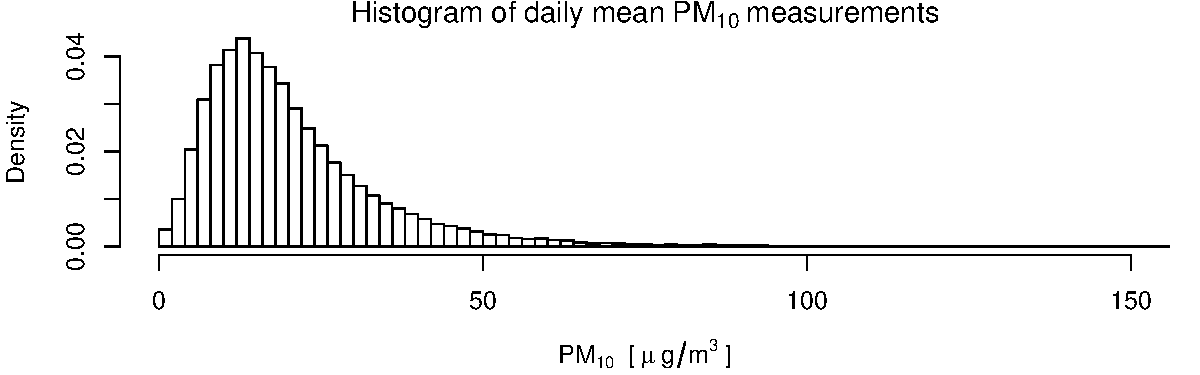
\includegraphics[width=0.95\textwidth]{hist_PM10.pdf}
\caption{Histogram of the daily mean $\rm{PM}_{10}$ rural background concentrations across Europe during the year 2005. 60 observations extend beyond the plot up to approximately 400 $\rm{\mu g/m^3}$.\label{fig:histPM10}}
\end{figure}

\subsubsection*{Marginal distributions $F_{s}$ and $G_{s}$}
We fit marginal distributions for each location $s\in\mathcal{S}$ based on the time series leading to margins $F_s$ and $G_s$ for daily mean $\rm{PM}_{10}$ measurements and EMEP model estimates respectively. This leads to a slightly less general set-up as introduced earlier where the marginal distributions might as well change over time. Using the \pkg{evd} \proglang{R}~package \citep{Stephenson2002}, a generalized extreme value distribution is automatically fitted to each station's time series of $\rm{PM}_{10}$ and the EMEP model estimates. The assumptions of a single marginal distribution describing all stations could not be verified for either variable, as too many stations rejected these distributions in a Kolmogorov–Smirnov test. Obviously, these marginal distributions can only directly be fitted where we observed data. For an interpolation scenario, the marginals need to be extended towards prediction locations as well. Assuming that the marginal distributions change rather smoothly over space, we use two different models based on spatial proximity. One relies on a linear model incorporating the locations' coordinates and altitude followed by an inverse distance weighted interpolation of the residuals and the second one uses only inverse distance weighted means of the local neighbourhood's marginal parameters as estimates. Both approaches only use the spatially closest 9 locations for the inverse distance weighted means. Even though the spatio-temporal field we are modelling is not assumed to be stationary, we assume that the local dependence structure is the same all over Europe and can sufficiently be described by a station's 9 strongest correlated neighbours from up to 4 preceding time steps. In the following code snippets, we assume \code{EU_RB_2005} to be a spatio-temporal full data frame (class \code{STFDF}, see the documentation of \pkg{spacetime} \citep{Pebesma2012} for details) that holds the already station-wise marginal transformed data and model estimates denoted as \code{marPM10} and \code{marEMEP} respectively.

\subsubsection*{Covariate copula $C_{ZY}$}
Starting with the covariate copula $c_{ZY}$, we investigate the correlation structure of the daily mean $\rm{PM}_{10}$ measurements and EMEP model estimates over time. Figure~\ref{fig:corPM10vsEMEP} illustrates how the strength of correlation and the dependence structure changes throughout the year 2005. We use weekly correlations (red line in Figure~\ref{fig:corPM10vsEMEP}) averaging out a great deal of variation, but largely maintaining the changes over time. The copula families are selected among the elliptical Gaussian and Student and the Archimedean Clayton, Gumbel, Frank \citep{Nelsen2006} and Joe \citep{Joe1997} copula families as indicated by the black line segments in Figure~\ref{fig:corPM10vsEMEP}. The marginal independence of Kendall's tau ensures that this strength of dependence is the same for the marginal transformed as well as the raw data. This temporally changing covariate copula needs to be encoded as function taking the current spatio-temporal indices and returning a copula object:

\begin{Schunk}
\begin{Sinput}
R> library("spcopula")
R> coVarCop <- function(stInd) {
+    week <- min(ceiling(stInd[2] / 7), 52)
+    copulaFromFamilyIndex(weekCop[[week]]$family, weekCop[[week]]$par, 
+                          weekCop[[week]]$par2)
+  }
\end{Sinput}
\end{Schunk}

\begin{figure}
\center
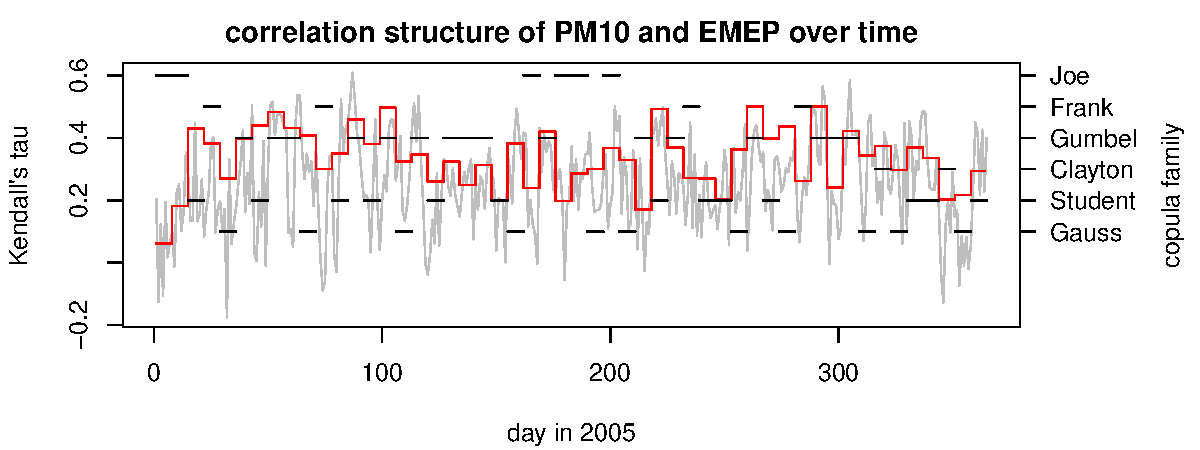
\includegraphics[width=0.95\textwidth]{PM10_EMEP_correlation.pdf}
\caption{Correlation structure of daily mean $\rm{PM}_{10}$ measurements and EMEP predictions over time. The grey line indicates daily Kendall's tau values while the red step function describes weekly empirical Kendall's tau values. The black line segments denote the copula family best describing the dependence structure during each week for the given empirical correlation (without any particular ordering).\label{fig:corPM10vsEMEP}}
\end{figure}

\subsubsection*{Spatio-temporal bivariate copula}

For the estimation of the spatio-temporal bivariate copula, we follow the suggested procedure from Section~\ref{sec:estimation} and start by grouping the data into spatial bins for five temporal lags (i.e., the same and first to fourth preceding day). For each spatio-temporal lag, the mean distance of all involved pairs and their Kendall's tau are calculated by:
\begin{Schunk}
\begin{Sinput}
R> stBins <- calcBins(EU_RB_2005, "marPM10", nbins = 40, tlags = -(0:4))
\end{Sinput}
\end{Schunk}
The resulting object \code{stBins} is of type \code{list} with entries \code{meanDists} denoting the mean spatial distance of spatio-temporal bins, \code{lagCor} holding the correlation values per spatial bin and temporal lag and \code{lags} providing spatial and temporal indices to access the data from the underlying \code{STFDF}. Correlation functions (here five polynomials of degree three each) can directly be fitted to the above output and are joint in a spatio-temporal dependence function (\code{stDepFun}) through:
\begin{Schunk}
\begin{Sinput}
R> stDepFun <- fitCorFun(stBins, rep(3, 5), tlags = -(0:4))
\end{Sinput}
\end{Schunk}
Figure~\ref{fig:stCopula} illustrates the empirical values of Kendall's tau per spatial bin and temporal lag alongside with the corresponding polynomial fits. These polynomials describe how the strength of dependence changes with spatial and temporal distance. Following the estimation procedure, we need to investigate how the dependence structure, i.e., the copula families change for different spatial bins and temporal lags. The polynomials describing Kendall's tau in terms of distance are used to derive the parameter of a set of copula families and their log-likelihood is calculated per spatial bin and temporal lag. In case the relationship between Kendall's tau and the copula parameters is not unique, the parameter is optimised based on a log-likelihood approach
restricted under the desired value of Kendall’s tau. The function \code{loglikByCopulasStLags} calculates the log-likelihoods per spatial bin and temporal lag additionally returning the evaluated copula:

\begin{figure}
\center
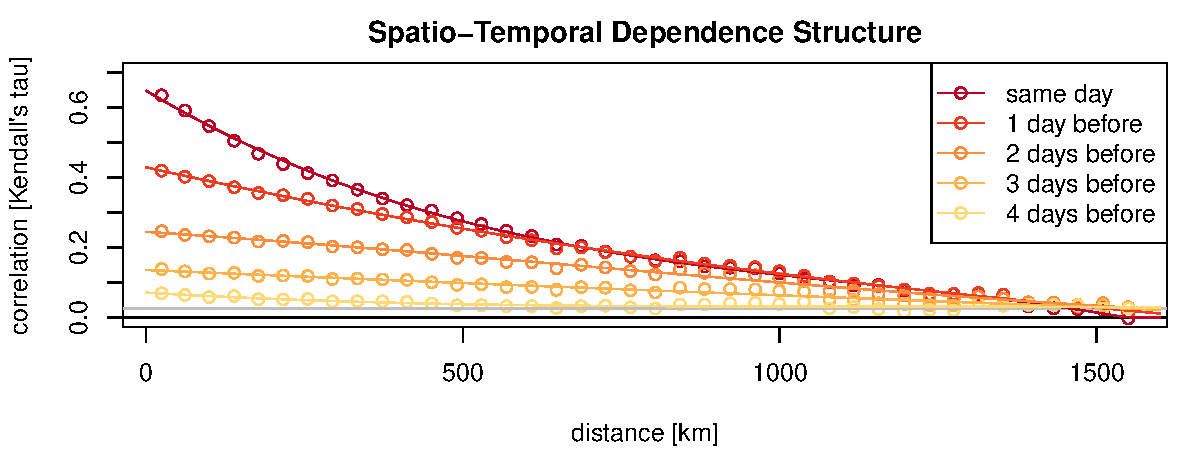
\includegraphics[width=0.95\textwidth]{correlogram.pdf}
\caption{Empirical and modelled values of Kendall's tau for the bivariate spatio-temporal copula over five temporal lags.\label{fig:stCopula}}
\end{figure}

\begin{Schunk}
\begin{Sinput}
R> families <- c(normalCopula(0), tCopula(0),
+                claytonCopula(0), frankCopula(1), gumbelCopula(1), 
+                joeBiCopula())
\end{Sinput}
\end{Schunk}

\begin{Schunk}
\begin{Sinput}
R> loglikTau <- loglikByCopulasStLags(stBins, EU_RB_2005, families,
+                                     stDepFun)
\end{Sinput}
\end{Schunk}


Copula families considered for the bivariate spatio-temporal copula (\code{families}) include the elliptical Gaussian and Student copulas, the Archimedean Clayton, Frank, Gumbel \citep{Nelsen2006} and Joe \citep{Joe1997} copulas. % and two copulas with cubic and quadratic sections where the last one is an asymmetric copula \citep[Example 3.16]{Nelsen2006}. 
The best fitting copula family is selected based on the highest log-likelihood. % while for the temporal lag of zero, the asymmetric copula is not considered assuming a spatially isotropic model:

\begin{Schunk}
\begin{Sinput}
R> bestFitTau <- lapply(loglikTau, 
+                       function(x) apply(apply(x$loglik, 1, rank),
+                                         2, which.max))
\end{Sinput}
\end{Schunk}

\begin{table}[bt]
\tabcolsep 1.8pt
\center\small
\begin{tabular}{l|ccccccccccccccc}
 & \multicolumn{15}{c}{Spatial lag} \\ \hline
\rule{0pt}{12pt}ID & 1 & 2 & 3 & 5 & 6 & 7 & 22 & 23 & 25 & 26 & 27 & 28 & 29 & 30 & 33 \\
mean dist. [km] & 25 & 61 & 99 & 177 & 216 & 255 & 843 & 881 & 961 & 999 & 1038 & 1079 & 1117 & 1156 & 1274 \\ \hline
\rule{0pt}{12pt}$\Delta = 0$      &  t  &  G  &   t & \dots &  t   & G&\multicolumn{3}{c}{\dots}& G &    F   &    N   &    F   &     N  & \dots \\
$\Delta = -1$     & G  &\multicolumn{5}{c}{\dots}   &  G  &F&\multicolumn{2}{c}{\dots}&F&  N   &    F   &     N  &    N   \\
$\Delta = -2$     & G  &\multicolumn{7}{c}{\dots}                       & G   &   N    & \multicolumn{5}{c}{\dots} \\
$\Delta = -3$     & G  &\multicolumn{10}{c}{\dots}                                                      & G     &   N  & \multicolumn{2}{c}{\dots} \\
$\Delta = -4$ &G&\multicolumn{2}{c}{\dots}&G&J&\multicolumn{4}{c}{\dots}&J& G &     G    &   N  & \multicolumn{2}{c}{\dots}
\end{tabular}
\caption{Spatio-temporal bivariate copula family configuration for the first 33 spatial lags as suggested by the highest log-likelihoods. $\Delta$ indicates the time lag and the copula families are abbreviated as follows: N = Gaussian, t = Student, C = Clayton, F = Frank, G = Gumbel and J = Joe.\label{tab:copFamilies}}
\end{table}

In this application, the copula families change rather little and the Gumbel copula family (compare Figure~\ref{fig:copula_densities}) dominates the dependence structure. The spatio-temporal bivariate copula configuration is listed in Table~\ref{tab:copFamilies}. Using the earlier fitted polynomials and this selection of copula families, the convex combination of copulas (Equation~\ref{eq:spCop} and the following paragraph) can now be composed to a spatio-temporal bivariate copula. The selected copula fits \code{listCops} and the representative distances \code{listDists} are provided as lists with one entry for each temporal lag. Each of this entries contains a list of copulas in spatially ascending order:
\begin{Schunk}
\begin{Sinput}
R> distSelect <- function(x) {
+    stBins$meanDists[sort(unique(c(which(diff(x) != 0),
+                                   which(diff(x) != 0) + 1, 1, 40)))]
+  }
R> listDists <- lapply(bestFitTau, distSelect)
\end{Sinput}
\end{Schunk}

\begin{Schunk}
\begin{Sinput}
R> famSelect <- function(x) {
+    families[x[sort(unique(c(which(diff(x) != 0),
+                             which(diff(x) != 0) + 1, 1, 40)))]]
+  }
R> listCops <- lapply(bestFitTau, famSelect)
\end{Sinput}
\end{Schunk}

As the corresponding Kendall's tau value used to tune the bivariate copula's parameter is calculated for each spatio-temporal distance, the above components and the spatio-temporal dependence function define the bivariate spatio-temporal copula \code{stBiCop}:

\begin{Schunk}
\begin{Sinput}
R> stBiCop <- stCopula(components = listCops, distances = listDists, 
+                      tlags = -c(0:4), stDepFun = stDepFun)
\end{Sinput}
\end{Schunk}

\subsubsection{Joining vine copula}

For the further processing, the data needs to be rearranged in local neighbourhoods. In our application, we are interested in the nine strongest correlated neighbours. Typically, there is no easily identified metric selecting these and we start with a larger static neighbourhood structure following Figure~\ref{fig:stNeigh}. The function \code{reduceNeighbours} selects the $n$ strongest correlated neighbours as given in the third argument. To accomplish this, the spatio-temporal distances of the larger cubic neighbourhood are passed to the spatio-temporal dependence function \code{stDepFun} and the ones with the highest values are selected: 
\begin{Schunk}
\begin{Sinput}
R> stNeigh <- getStNeighbours(EU_RB_2005, var = "marPM10", spSize = 9, 
+                             tlags = -(0:4), timeSteps = 90, min.dist = 10)
R> stRedNeigh <- reduceNeighbours(stNeigh, stDepFun, 9)
\end{Sinput}
\end{Schunk}
This approach allows to drop missing values and to select the next best (i.e., next strongest correlated) available neighbour. The argument \code{spSize} denotes the number of locations at the current level including the central location. By setting \code{timeSteps} to 90, every location will only be used at 90 randomly assigned time steps as a centre of the neighbourhood. This way, only temporal chunks of five consecutive days are used reducing unwanted autocorrelation in the time series but reflecting the local temporal structure of the phenomenon. With \code{min.dist} one ensures that any pair of neighbours has a minimum spatial separation distance (here 10~m). 

The conditioning on the covariate EMEP and the evaluation of the spatio-temporal bivariate copula on the neighbours can be done separately. The spatio-temporal bivariate copula returns pseudo observations that are the values of the neighbours conditioned on the value of the central location ($u_{i|0}$ from Equation~\ref{eq:pseudoObs}) incorporating the spatio-temporal distances between these by

\begin{Schunk}
\begin{Sinput}
R> condData <- dropStTree(stRedNeigh, EU_RB_2005, stBiCop)
\end{Sinput}
\end{Schunk}

In a loop, the weekly varying copulas as depicted in Figure~\ref{fig:corPM10vsEMEP} and encoded as \code{coVarCop} are used to relate the marginal transformed variable $\rm{PM}_{10}$ with its covariate EMEP. In order to select the appropriate copula, the spatio-temporal indices need to be retrieved from the larger neighbourhood:

\begin{Schunk}
\begin{Sinput}
R> condCoVa <- condCovariate(stNeigh, coVarCop)
\end{Sinput}
\end{Schunk}

 Binding this conditioned column \code{condCoVa} with the conditioned data from the spatio-temporal bivariate copula \code{condData} yields the data set for the upper vine estimation through the generic function \code{fitCopula}:

\begin{Schunk}
\begin{Sinput}
R> secTreeData <- cbind(condCoVa, as.matrix(condData@data))
R> vineFit <- fitCopula(vineCopula(10L), secTreeData)
\end{Sinput}
\end{Schunk}

Following the initial definition of the function \code{fitCopula}, the copula family that should be fitted needs to be provided as copula object. The call of the constructor \code{vineCopula} with an integer as argument (denoting the dimension) generates a canonical vine with independence copulas. The fitting routine sequentially selects the best fitting copula from a versatile set of copulas (see the documentation of \pkg{VineCopula}). The final spatio-temporal covariate vine copula is defined by:

\begin{Schunk}
\begin{Sinput}
R> stCVVC <- stCoVarVineCopula(coVarCop, stBiCop, vineFit@copula)
\end{Sinput}
\end{Schunk}

The cross-validation carried out to assess the goodness of fit of this spatio-temporal vine copula drops the complete time series of each location in turn and predicts this time series based on the neighbouring data. In this application, we predict the expected value as given in Equation~\ref{eq:expectation} of the time series for each moment in time. Prediction for a spatio-temporal target geometry \code{targetGeom} from the spatio-temporal vine copula is obtained by:

\begin{Schunk}
\begin{Sinput}
R> predNeigh <- getStNeighbours(EU_RB_2005, targetGeom, 
+                               spSize = 9, tlags = -(0:4),
+                               var = "marPM10", coVar = "marEMEP",
+                               prediction = TRUE, min.dist = 10)
R> predNeigh <- reduceNeighbours(predNeigh, stDepFun, 9)
R> stVinePred <- stCopPredict(predNeigh, stCVVC, list(q = qFun), 
+                             method = "expectation")
\end{Sinput}
\end{Schunk}

Where the argument \code{method} selects from the prediction methods \code{expectation} and \code{quantile} as given in Equation~\ref{eq:expectation} and Equation~\ref{eq:quantile} respectively. The default quantile is the median, but any fraction between 0 and 1 can be assigned to an argument \code{p}. This can also be used for simulation purposes, as simulated values can be obtained through uniform distributed fractions assigned to \code{p}.

\section{Results and discussion}
\label{sec:discussion}

Performing a cross-validation by leaving one complete station time series out in turn, the performance of this approach is assessed. Table~\ref{tab:cross-validation} lists the results of a cross-validation using the expectation predictors for the newly presented spatio-temporal covariate vine copula approach (STCV) for different margins, a STCV solely composed out of Gaussian copulas and the simpler spatio-temporal copula presented in \citet{Graler2012a}. Additionally, results of a cross-validation for an approach based on spatio-temporal metric residual kriging with an underlying log-linear regression of the same data set but incorporating 100 nearest neighbours \citep{Graler2012} is presented. In the case where the marginals refer to \emph{local GEV}, the station-wise estimates are used. This is only possible in the case of a cross-validation as in a typical prediction or simulation application one would not have this extra knowledge about the margins. This can be seen as a very good model of the marginals across space as the distributions of the margins are still not known, but extra data is used to estimate them. Hence, in a realistic cross-validation scenario, an additional model on the marginal distributions' parameters needs to be used. Here, we fitted two models for each of the three parameters. One using a linear model including coordinates and the station's altitude and performing a inverse distance weighted interpolation on the residuals of the spatially closest 9 neighbours (denoted \emph{lm+IDW}) and another using only an inverse distance weighted interpolation of the spatially closest 9 neighbours (denoted \emph{IDW}). The major benefit in Table~\ref{tab:cross-validation} is due to the additional knowledge on the marginal distribution functions. A smaller improvement could be made for the STCV using the lm+IDW marginal distributions but these statistics are within the same order of magnitude as the earlier presented spatio-temporal vine copula or the kriging predictor. These results underline how important it is to obtain good fits of both, the copula and the marginal distributions. 

\begin{table}
\center
\begin{tabular}{ll|rrrr}
Dependence model & Margin & RMSE & MAE & ME & COR \\ \hline 
\rule{0pt}{14pt}STCV $\widehat{Z}_m$ & local GEV & 8.53 & 4.61 & -0.05 & 0.84 \\
Gaussian STCV $\widehat{Z}_m$  & local GEV & 8.65 & 4.59 & 0.08 & 0.83 \\
STCV $\widehat{Z}_m$ & lm+IDW GEV& 10.12 & 5.79 & 0.17 & 0.76 \\
STCV $\widehat{Z}_m$ & IDW GEV&  10.82 & 6.26 & 0.14 & 0.72 \\
metric res. kriging & log linear reg. & 10.67 & 6.16 & 0.47 & 0.74 \\
sp.-temp. vine $\widehat{Z}_m$ & global GEV & 11.20 & 6.95 & -0.73 & NA 
\end{tabular}
\caption{Cross-validation results comparing the expectation spatio-temporal estimators for the newly presented spatio-temporal covariate vine copula with different margins, the spatio-temporal vine copula as in \citet{Graler2012a} and results from an earlier study by \citet{Graler2012} using kriging based approaches assuming a metric spatio-temporal covariance structure of the residuals of log-linear regression.}\label{tab:cross-validation}
\end{table}

\begin{figure}
\center
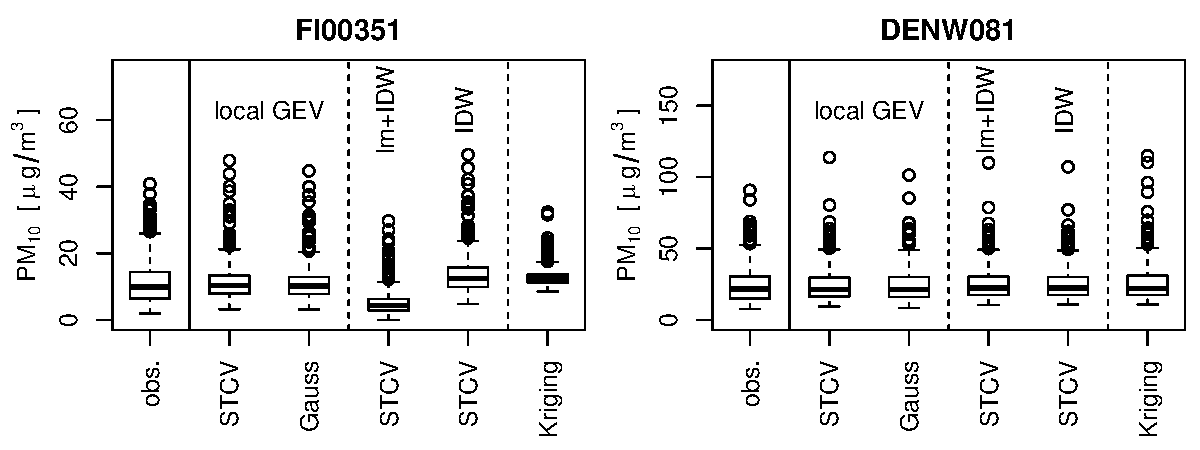
\includegraphics[width=0.95\textwidth]{BoxPlots.pdf}
\caption{Boxplots comparing the different predictors with the observed values at two stations. The Finish one (left) is an isolated location while the German one (right) is situated in a rather dense network.\label{fig:boxplots}}
\end{figure}

Besides looking at pure cross-validation statistics, it is important to consider the reproduction of the full distribution. Figure~\ref{fig:boxplots} shows boxplots of the observed versus modelled time series at two exemplary stations in Finland (FI00351) and Germany (DENW081). The Finish one is far away from any other station while the German one is situated in a rather dense network. Looking at many more plots of this kind for several stations (not shown) reveals that the copula based methods are rather close to each other and represent the original data quite well. Within the copula approaches, the full cross-validations \emph{lm+IDW} and \emph{IDW} have the largest deviations. The kriging based approach turns out to predict too large as well as too small ranges of values depending on the single station with a notable shift of the median at some stations. The issue of failing to reproduce the time series at isolated locations detected in the first application of a simpler spatio-temporal vine copula \citep{Graler2012a} could be overcome with the local GEV margins and considerably improved with \emph{lm+IDW} and \emph{IDW}. In Figure~\ref{fig:FI00351} the same temporal subset is plotted as in Figure~3 of \citet{Graler2012a} but the copula approaches are now able to follow the time series more closely than the kriging based predictor. 

\begin{figure}
\center
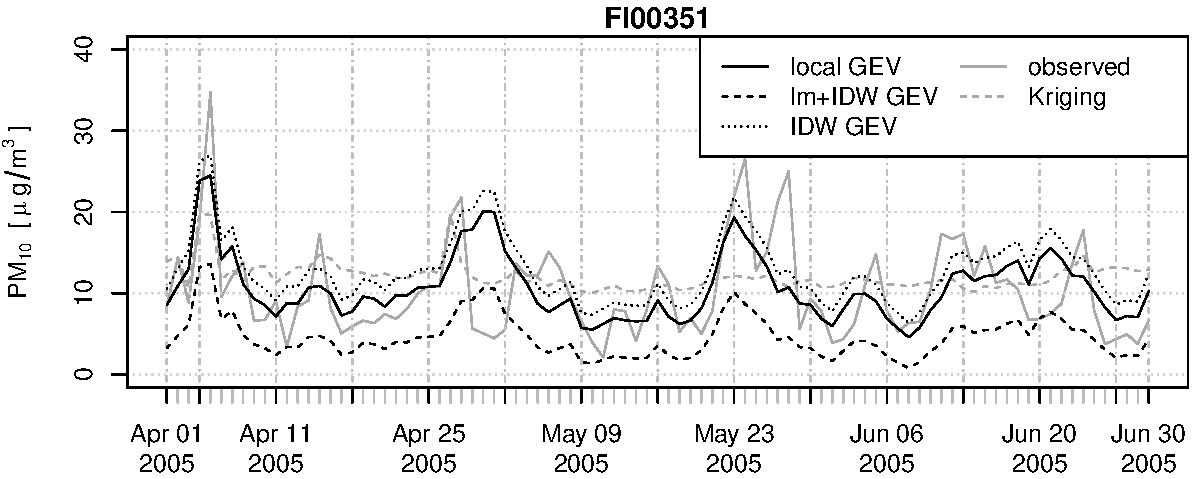
\includegraphics[width=0.95\textwidth]{FI00351_ts.pdf}
\caption{A subset of the time series at a Finish station comparing different predictors.\label{fig:FI00351}}
\end{figure}

An advantageous feature of the copula approaches is their ability to provide potentially more reliable uncertainty assessments. Different from kriging, the prediction variance does not only depend on the spatio-temporal configuration of the locations, but also on the predicted value. Due to the nature of kriging, every conditional distribution is again a normal distribution. This is different for the copula approaches where the predictive density can take any form and the fitted marginal distribution functions ensure a reasonable range of possible values. Figure~\ref{fig:predDensity} illustrates the predictive densities at two different days at location DENW081. Note that besides the position also the shape of the prediction CDFs changes.

\begin{figure}
\center
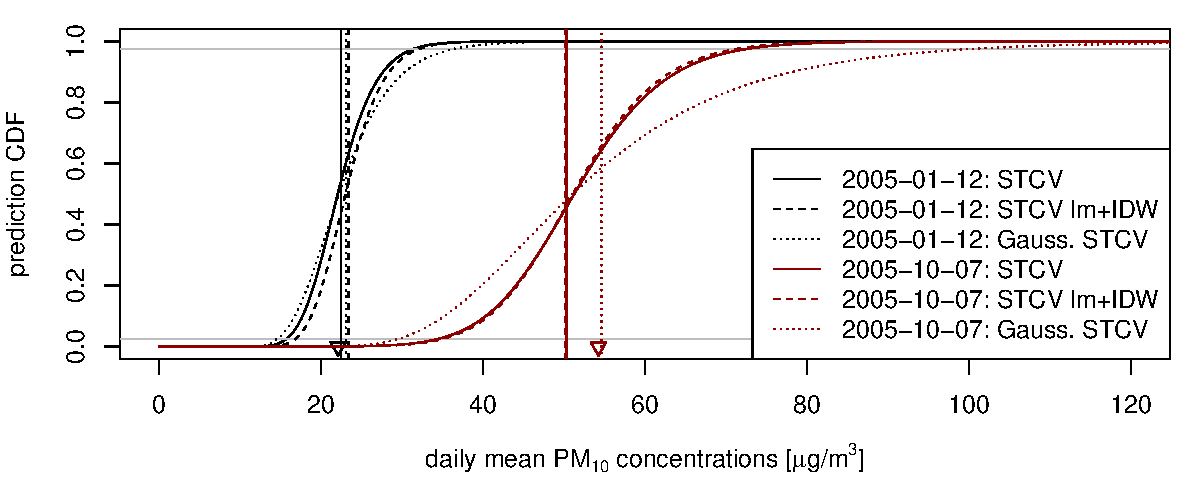
\includegraphics[width=0.95\textwidth]{condPredCDF.pdf}
\caption{Prediction CDFs for station DENW081 at two different days in 2005. The vertical lines denote the predicted while the symbols on the x-axis indicate the observed value. The two horizontal lines denote the cumulative probabilities $0.025$ and $0.975$ easing the  assessment of the $95\%$-confidence intervals.\label{fig:predDensity}}
\end{figure}

Even though simulating from a spatio-temporal random field modelled by a spatio-temporal covariate vine copula has not been shown in this application, it is readily done by not predicting for a constant cumulative distribution value but a random $p$ in $\widehat{Z}_p(s,t)$ for each location $(s,t)$. In a conditional simulation, it is a modellers choice to which degree already sampled and closer locations are preferred over conditioning but further apart locations in the local neighbourhood. Modelling the spatio-temporal random field only locally requires a simulation along a random path. To avoid clustering effects along this path, one might start with simulations on a regular coarse subset of the target locations and simulate subsequently on finer regular subsets \citep{Gomez-Hernandez1991}.

Computational cost of the vine copula approaches might be a burden where results need to be generated very fast. The prediction of approximately 70000 values in the presented cross-validation takes a bit more than a day on a common laptop. No efforts have been made to speed up the execution for example by making use of parallel evaluation. 

\section{Conclusions}
\label{sec:conclusion}
The \pkg{spcopula} package allows the modelling of spatial and spatio-temporal random fields by vine copulas. An earlier study \citep{Graler2014} demonstrated the potential of spatial vine copulas for heavily skewed spatial random fields. The newly presented spatio-temporal covariate vine copula improves the interpolation of particulate matter compared to earlier spatio-temporal vine copulas \citep{Graler2012} and linear geostatistical approaches. Nevertheless, the current bottleneck of the presented application is the flexible modelling of marginal distributions. This became evident by the presented cross-validation using extra knowledge about the margins.

The bivariate spatio-temporal copulas on the first tree mainly incorporate a Gumbel copula indicating a stronger dependence in the tails, a feature that is not available in a Gaussian set-up. Each spatio-temporal location has its own individual conditional distribution that is used for prediction. Different from kriging where each predictive distribution is again Gaussian, the conditional distributions of the STCV can take any form, potentially providing more realistic uncertainty estimates. Simulating from the modelled random field is possible and has been implemented in the presented package. A disjoint modelling of margins and dependence structure introduces a large flexibility to define a random fields distribution. Nevertheless, it is very important to obtain good models for both components for a successful application.

\clearpage
\section*{Acknowledgements}
This research has been funded by the German Research Foundation (DFG) under project number PE 1632/4-1.

\bibliography{bib_spcopula}

\end{document}
